\documentclass[11pt]{article}
%Required: You must have these
\usepackage{graphicx}
\usepackage{tabularx}
\usepackage{natbib}

\usepackage{array}
\usepackage{amsmath}
%\usepackage[backend=bibtex]{biblatex}
\setkeys{Gin}{width=0.8\textwidth}
%\setlength{\captionmargin}{30pt}
\setlength{\abovecaptionskip}{10pt}
\setlength{\belowcaptionskip}{10pt}
\topmargin -2.5cm 
\oddsidemargin -0.04cm 
\evensidemargin -0.04cm 
\textwidth 16.59cm
\textheight 23.94cm 
\parskip 7.2pt 
\renewcommand{\baselinestretch}{1.2}
\parindent 0pt
\renewcommand{\thetable}{S\arabic{table}}
\renewcommand{\thefigure}{S\arabic{figure}}
\usepackage{lineno}
\bibliographystyle{..//refs/styles/besjournals.bst}
\usepackage{xr-hyper}
\externaldocument{periodicity2022rev}
\externaldocument{FE_rev_resp_partII}

%\usepackage{hyperref}
\title{Supporting Information: Experimental designs for testing the interactive effects of temperature and light in ecology: the problem of periodicity }
\date{}
\begin{document}
\maketitle
%\subsection{Light and temperatre and spring phenology}
%Here a very brief (one or two paragraph) overview of how light and temperature influence spring phenology. Keep it basic (Warming accelerate phenology, photoperiod might be a threshold), acknowledge %chilling is important too, but our example won't really focus on it. Leave some open questions about their interactive nature.
%Lizzie, I need help  making/checking this.\\
%I ran countintxns.R, now on main ospree branch.\\
%I think line 78 tells me how many studies could test forcing x photoperiod interactions (15)\\
%Line 92-94 tells me how many might have periodicity issues (4 datasets or 7 experiments)\\

%That seems too small. Why do I think this?  Co-variation is an issue even if you don't care about forcing (e.g. most falusi papers are interested in photoperiod effect, and while they do not use forcing as a treatment, they vary day and night temperature, so any photoperiod effect the estimate could be a secret forcing effect). I think the big Zohner study would have this problem too. Basically, anytime you are testing the effect of photperiod and varying thermoperiod you have a problem. I am a bit overwhelmed by the countintxns.R code. Can this be investigate easily based on pre-existing script? bbstanallsppmodelcountinxns.csv say there are 21 studies that vary thermoperiodicity with some other treatment.
\section*{Figures:}
 \begin{figure}[h!]
    \centering
 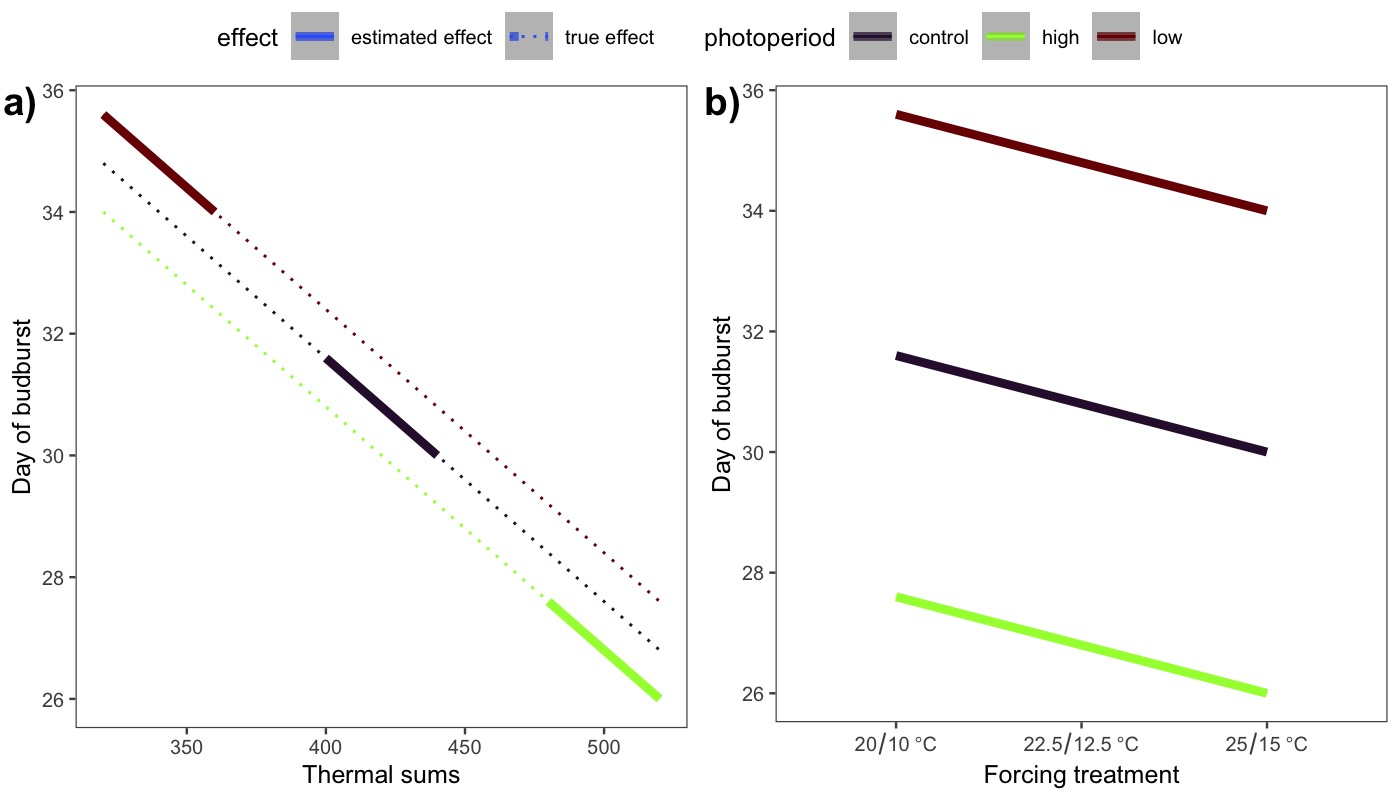
\includegraphics[width=.7\textwidth]{..//Plots/periodicity_figures/apparent4spp.jpeg}
    \caption{Estimated effects of photoperiod and forcing on spring phenology based on a simulated experiment in which the coupling of photoperiod and thermoperiod introduce an experimental covariation between three levels of temperature and light treatments. The dotted lines in \textbf{a)} depict the true effects of forcing at each photoperiod level, and the solid lines depict the estimated effects. \textbf{b)} depicts the estimated effects of forcing and photoperiod if the experimental covariation due to periodicity coupling in \textbf{a)} is unacknowledged.}
    \label{fig:suplines}
\end{figure}

\section*{Estimating the effects of experimental periodicity covariance mathmatically}
%Maybe Lizzie (or Megan) can write this part since they were the ones who did this math?
  % EMW: Putting this here for now, but can move some/all it to main text as needed. [] means I am not sure we need it, but I added it. 
%[See comments in tex file.] \\
When experimental designs couple thermo- and photo- periodicity and therefore, forcing and photoperiod treatments covary, they may incorrectly estimate the effects of forcing, photoperiod, and (for experiments with crossed designs) their interaction. While robustly testing the effect of this experimental covariation requires additional experiments, we can solve for its potential effect based on the geometry of the experimental design given several assumptions.

If we assume forcing and photoperiod effects are additive and linear (i.e., there is no interaction), then the treatments and their resulting effects occupy a plane, and we can solve algebraically for the separate effects of forcing and photoperiod.  If we replace the qualitative factor (high forcing/low forcing) by the quantitative effect of forcing (daily thermal sums) to properly account for the difference in forcing between short and long photoperiods, then the plane is defined on a three dimensional space with thermal sums on the $x$ axis, photoperiod on the $y$ axis, and the response on the $z$ axis. Given the assumption of no interaction, we can solve for the expected response if forcing and photoperiod were fully independent. 

Here, we work through an example based on the experiment described in \cite{Flynn2018}. First, we redefine the forcing treatment (20/10$^{\circ}$C vs. 15/5$^{\circ}$C) as thermal sums (degree hours) to reflect the duration and intensity of temperature to define the $x$ axis. The $y$ axis is defined by the photoperiod treatment levels (8 hours vs. 12 hours), and the $z$ axis is the response, defined as the change in days to budburst ($\Delta$) for this experiment. With these axes, we can use a system of three equations to define a plane (Equations 1-3), 

\begin{align}
ax_1+by_1+cz_1+d & =0\\
ax_2+by_2+cz_2+d & =0\\
ax_3+by_3+cz_3+d & =0
\end{align}

and take three points that define the main effects in the experiment (low forcing/short day, low forcing/long day, high forcing/short day; i.e., the effect of daylength holding forcing constant, and the effect of forcing holding daylength constant) as the three points that define the plane:
  
  \begin{align}
200a + 8b + 0 + d &= 0\\
240a + 12b+4.5c + d &=0\\
320a + 8b + 9c+ d &=0
\end{align}

where Equation 4 is the result of the low forcing, short day treatment where thermal sum ($x$) is 200 degree hours, photoperiod ($y$) is 8 hours, and change in days to budburst is 0; Equation 5 is the result of the low forcing, long day treatment ($x$ = 240 degree hours, $y$ = 12 hours, $z$ = 4.5 days); and Equation 6 is the result of the high forcing, short day treatment ($x$ = 320 degree hours, $y$ = 8 hours, $z$ = 9 days); \citep[see][Table S5]{Flynn2018}.  Algebraically, we simply solve for each unknown in turn. 

Solving Equation 4 for $d$ in terms of $a$ and $b$
  \begin{align}
200a + 8b + 0 + d & = 0 \text{ and solving for d yields:} \\
-200a - 8b & =  d  % setting c to 0
\end{align}
Now, we can solve for $c$ (in terms of $a$ and $b$) using our solution for $d$:
  \begin{align}
240a+12b+4.5c+(-200a - 8b) & = 0\\
-40/4.5a+4/4.5b & = c% simplified 
\end{align}
And similarly then solve for $a$ given our last set of coordinates and solutions for $d$ and $c$ (not shown). This yields:
  \begin{align}
a & =\frac{1}{5}b\\
c & =-\frac{8}{3}b\\
d & =-48b
\end{align}
Putting these back into the equation for a plane yields an overall equation to estimate the response $z$ (days) for any combination of $x$ (thermal sum) and $y$ (photoperiod):
  \begin{align}
z & = \frac{3}{40}x + \frac{3}{8}y-18
\end{align}
Usign this equation, we can calculate the response for an existing treatment, e.g., low forcing/short day where thermal sum ($x$) is 200 degree hours and photoperiod ($y$) results in the measured days to budburst of ($z$) as zero.  We can also calculate the expected response for a treatment that \textit{was not} included in the experiment, e.g., a short day thermal sum with a long day photoperiod, $x$ = 200 degree hours and $y$ = 12 hours, to calculate the expected change in days to budburst $z$,
\begin{align}
\frac{3}{40}*(200) + \frac{3}{8}*(8)-18 &=0\\ 
\frac{3}{40}*(200) + \frac{3}{8}*(12)-18 &=3 
\end{align}

showing that the effect of changing photoperiod from 8 to 12 hours \textit{without} a change in forcing---given our assumptions---is a 3 day advance in budburst.\\ 

Finally, we can calculate the response for high forcing/long day, given the assumption of no interaction:
  
  \begin{align}
\frac{3}{40}*(360) + \frac{3}{8}*(12)-18 &=13.5
\end{align}


\section*{Modeling methods}
To investigate the impact of experimental photo- and thermo- period covariance on the estimated effects of photoperiod and forcing cues on spring phenology, we used data from two published phenology studies: \cite{Flynn2018} and \cite{Buonaiuto:2021ug}. Both\linelabel{common1} studies used dormant twigs collected from Harvard Forest in Petersham, MA, USA (42.5314$^{\circ}$N, 72.1900$^{\circ}$W)  and exposed them to comparable photoperiod and forcing treatments levels---photoperiod for both studies: 12 vs. 8 hours; forcing: 20/10$^{\circ}$C vs. 15/5$^{\circ}$C day/night for \citet{Flynn2018}; 24/18$^{\circ}$C vs. 18/12$^{\circ}$C day/night for \citet{Buonaiuto:2021ug}---in full factorial growth chamber treatments. We subset each dataset to include only matching phenological observations, termed ``leaf expansion" or BBCH 11 \citep{Finn2007}, and\linelabel{common2} species. This data subset included 713 observations (n_{\cite{Flynn2018}}=384, n_{\cite{Buonaiuto:2021ug}}=329, n_{species}=7).

We estimated the effect of study design on parameter estimates with a Bayesian hierarchical mixed effect model with weakly informative priors. %While both experiments were designed to test for interactions between photoperiod and forcing, we did not include this interaction term in our model in order to match the assumption of non-interactivity in the math. 
We included forcing, photoperiod, study and their interactions as main effects, and species as a random effect. We ran the model using the R package ``brms" \citep{Burkner2018} on 4 chains with 2000 iterations and warmup of 1000 iterations for a total of 4000 posterior samples per parameter. The model is written below.

$leafexpansion_{[i]} \sim N(\alpha_{sp_{[i]}}+\beta_{study} $\times$ \beta_{forcing} $\times$ \beta_{photoperiod}, \sigma_y^2)$\\

We modeled the intercept ($\alpha$) at the species level using the formula:\\

$\alpha_{sp} \sim N(\mu,\sigma^2)$\\

%We note that the because the subset of overlapping data between the two studies is considerably smaller than it is not surprising that the relative effect sizes of photoperiod and forcing estimated here differ from those reported in the full, published studies.

%\begin{table}[ht]
%\centering
%\begin{tabular}{rrrrrrr}
%  \hline
% & Estimate & Est.Error & Q2.5 & Q25 & Q75 & Q97.5 \\ 
% \hline
%Intercept & 57.35 & 4.98 & 47.40 & 54.25 & 60.46 & 67.39 \\ 
% PHOTO & -3.28 & 0.38 & -4.03 & -3.54 & -3.03 & -2.51 \\ 
%  FORCE & -1.32 & 0.15 & -1.61 & -1.42 & -1.21 & -1.02 \\ 
% study & 12.22 & 2.49 & 7.47 & 10.50 & 13.96 & 17.02 \\ 
%PHOTO:study & 2.27 & 0.66 & 1.02 & 1.82 & 2.73 & 3.57 \\ 
%FORCE:study & -1.74 & 0.39 & -2.49 & -2.00 & -1.47 & -1.00 \\ 
% \hline
%\end{tabular}
%\label{tab:esty}
%\caption{Main effect estimates from a Bayesian hierarchical model comparing coupled and uncouple experimental design. In this case, interactions with study represent the uncoupled estimates.}
%\end{table}

\bibliography{..///refs/periodicity.bib}

\end{document}